\chapter{Scope of research} \label{cha:Objectives}

\section{Introduction} \label{cha:Research-questions}
Published studies in the area of low-thrust trajectory optimisation, such as \textcite{Petropoulos2007}, frequently conclude that available optimisation techniques require further improvement, particularly in the areas of global search and modelling fidelity. Thus the most important question in this research project is how best to optimise a low-thrust trajectory. 

\begin{figure}
\centering
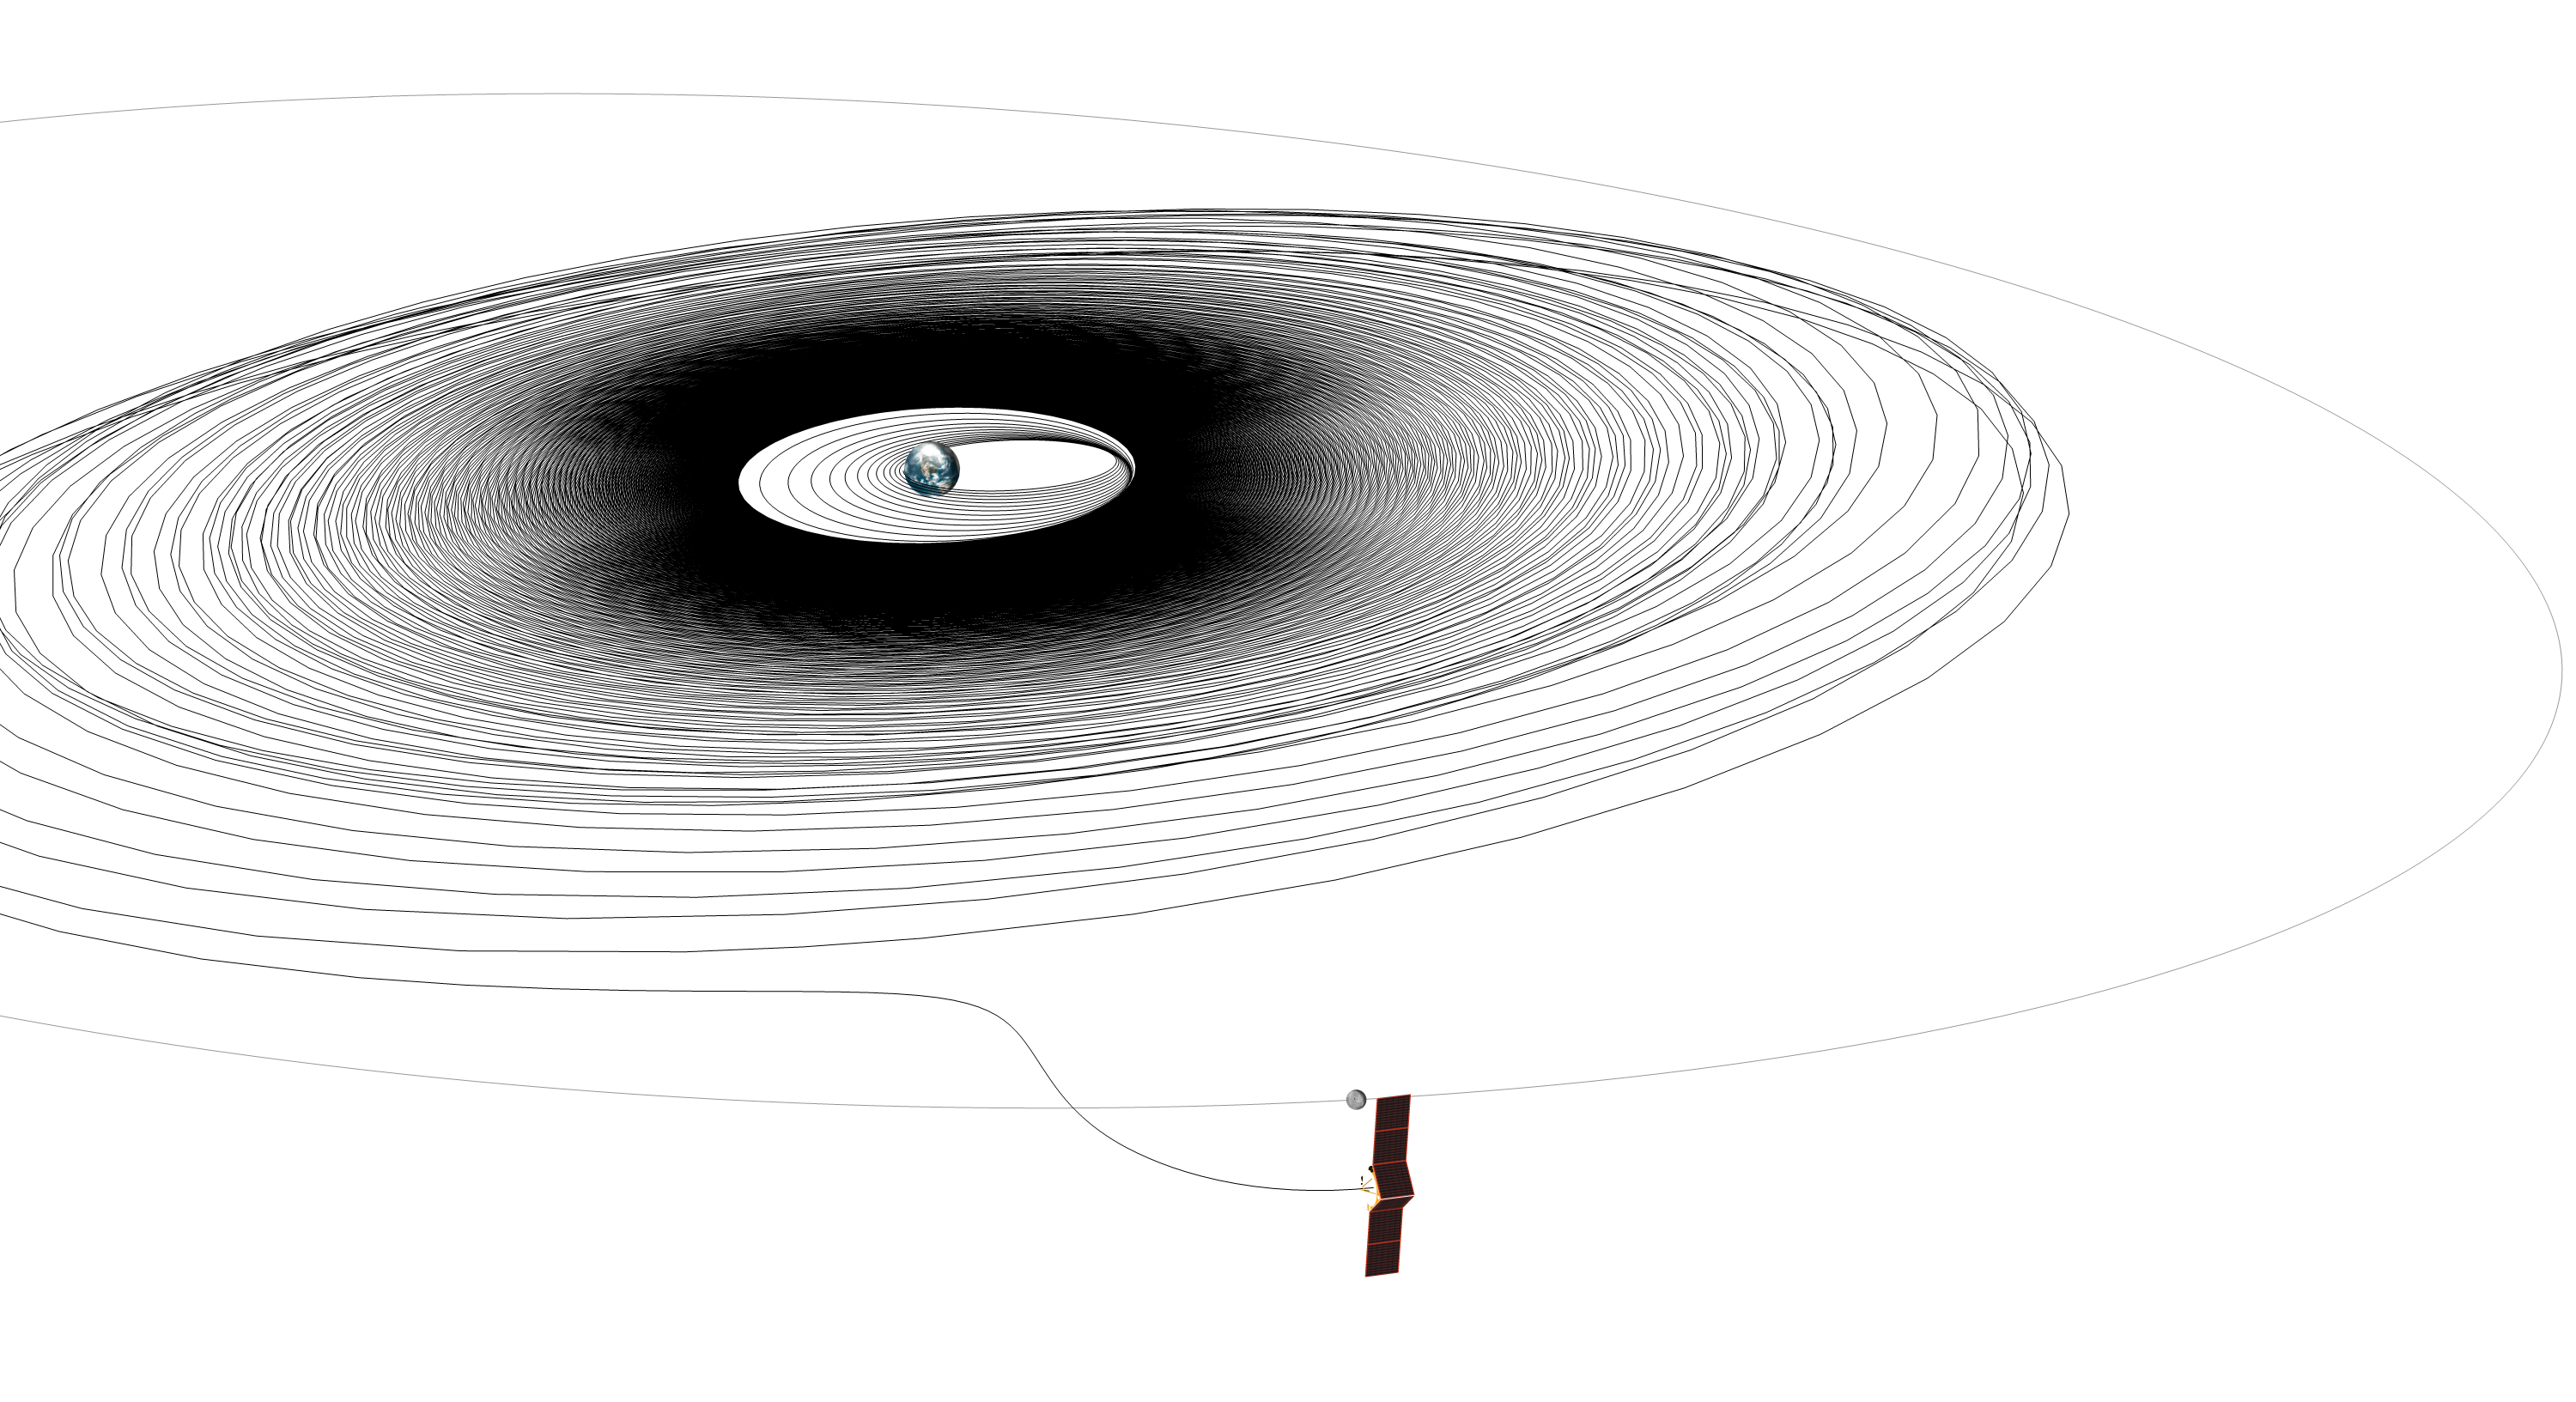
\includegraphics[width=\textwidth]{Images/BW1_Transfer.png}
\caption{A simplified trajectory prepared  for demonstration purposes early in the \emph{Kleinsatelliten} program.} \label{fig:Early-trajectory}
\end{figure}

The primary objective of optimising a low-thrust trajectory leads into two very interesting secondary outcomes of this project. Firstly, investigating the severity of perturbing forces on the spacecraft during transit, and to what extent they can be exploited. Secondly, developing a robust model to include a variety of non-linear trajectory constraints in the optimisation process.

% Optimise trajectory
\section{Optimisation of a low-thrust trajectory} \label{sec:Optimisation-objective}

The broad objective of optimising a low-thrust trajectory was broken down into the following tasks.

\begin{enumerate}
  \item Derive an appropriate model for the spacecraft, moving within a realistic space environment.
  \item Examine optimisation techniques and select one appropriate to this scenario.
  \item Explore different initial guesses for the optimisation, based on knowledge of orbital mechanics and exploitation of perturbing forces.
  \item Apply non-linear constraints to the optimisation.
\end{enumerate}

% Orbital mechanics
\subsection{Modelling} \label{sub:Modelling-task}

A complete description of the spacecraft and space environment model is presented in \autoref{cha:Orbital-dynamics}. Although there are multiple solutions available for each modelling hurdle, there are fairly well established best-practice solutions for the high fidelity modelling required over the long durations associated with low-thrust missions.

% Optimisation techniques
\subsection{Investigation of optimisation techniques} \label{sub:Optimisation-techniques}

Optimisation techniques suitable for trajectory optimisation were examined. Reviewed literature repeatedly cited the inadequacies of existing search methods as a major problem with existing optimisation methods, as addressed in detail in \autoref{cha:Literature-review}. In particular, it was noticed that previous optimisations generally ignore non-linear thruster constraints, due to the additional complexity and stiffness they add to the optimisation problem. Therefore finding a computationally efficient way to include non-linear constraints over long time spans was essential to the suitability of the optimisation techniques used for this mission.
 
% A thorough review of optimisation techniques is presented in Section \ref{cha:Optimisation}.

% Initial guesses
\subsection{Exploring different initial guesses} \label{sub:Initial-guesses}

Most optimisation techniques require an initial guess of the solution to be input into the algorithm, from whence they can improve their objective function. Existing search methods often have strong dependencies on the initial guess, as adressed frequently in literature such as \textcite{Dachwald2005}. Consequently it is important to investigate the performance of the optimisation under a variety of initial guesses. Based on orbital mechanics theory, a number of potentially optimal scenarios were investigated in this thesis, as outlined in \autoref{cha:Method}. These were then compared to a number of randomly chosen initial guesses, to determine the breadth of the basin of convergence and the ability of the optimiser to handle multiple basins. Additionally a number of severely sub-optimal initial guesses were examined.

% Model nonlinear constraints
\subsection{Application of non-linear constraints} \label{sub:Model-non-linear-constraints}

There are a number of very unique constraints on \BW. The thrusters produce substantially less thrust than modelled in most previous studies, resulting in a much narrower range of possible trajectories. The craft used in this program is also very limited by onboard power storage. This is yet another practical engineering issue barely considered in existing literature. Every few hours the craft must rotate to point its solar panels towards the Sun, and recharge its batteries. Once fully charged, it then rotates back to continue thrust vectoring for guidance control. Consequently the optimisation model must allow for variable thrust, including the ability to constrain thrust magnitude (to zero) at certain times. Developing a method to optimise intermittent thrust profiles like this will ensure the theoretical research of trajectory optimisation is applicable to real spacecraft.

First, a highly simplified low-thrust lunar trajectory was developed. This assisted in developing an initial guess for the final optimisation. From this state, the optimiser was developed to include more complex constraints. Coast phases were introduced to the existing constant-thrust profile, producing a bang-bang control scenario. Then the length of these coasting and thrusting phases was released, followed by the magnitude of the thrust. The electric power consumed during a thrust phase was modelled, with the constraint that it cannot drop below zero. An approximation of power generated by the solar panels was implemented, and then improved based on sunlight angle of incidence, Earth shadow and solar panel decay. This technique identified coasting phases required for recharging the spacecraft, providing constraints on the Attitude Control System (ACS). Propellant use was modelled, based on the thrust profile and constrained by power availability. Reaction wheel desaturation will be required to improve the fuel usage model, although this improvement is dependent on other project members working on the ACS and consequently has not been addressed.

% Investigate perturbations
\section{Investigation of perturbations} \label{sec:Perturbation-objective}

This project provides a rare opportunity to actually test a low-thrust trajectory in orbit. Due to the prohibitive cost of space exploration, most studies of this nature are purely academic. Academic studies such as \textcite{Betts2000} often simplify or neglect the more awkward perturbing forces acting on the spacecraft such as solar radiation and inhomogeneous gravity fields, for the sake of elegant mathematical solutions. The combination of very-low-thrust and the fact that the trajectory resulting from this study will actually be flown, requires that it take into account a much greater range of possible perturbations than most previous studies. The question of how significant these perturbations are, and particularly to what extent they may be exploited to reduce the effort needed to propel the spacecraft towards the Moon, may greatly affect the final launch.

To address this question, once a robust model was developed for the trajectory optimisation, the impact of perturbations on the trajectory was investigated. This objective was required to highlight two major characteristics of the trajectory: firstly, the robustness of the trajectory in the event of unanticipated perturbations, and secondly whether anticipated perturbing forces may be exploited to propel the spacecraft.

%The sensitivity of the trajectory was examined by introducing deterministic and stochastic inputs into variables such as the thrust angles, magnitudes, and gravitational perturbations, to simulate errors in the spacecraft control system, non-linearities in the thruster output, or unknown gravitational influences, to ensure that the proposed theoretical thrust regimes are applicable to real-world spacecraft. The magnitude of these error inputs was determined through consultation with experts on each of the sub-systems, as a percentage of the intended input. Additionally, the trajectory was simulated with errors of increasing magnitude to determine mission failure scenarios. Contingency trajectories will have to be determined for these cases, such as a single engine failure.

%Anticipated, predictable perturbing forces may be used to help propel the spacecraft towards the Moon. 
It is well known from interplanetary trajectories such as those presented by \textcite{Petukhov2007} that a large amount of propulsive effort can be saved by exploiting gravitational assists. Some textbooks, such as \textcite{Kemble2006}, and other publications such as \textcite{Letterio_thesis} discuss the possibility of exploiting the Moon's gravity in a series of lunar \enquote{resonances} to assist a low thrust lunar transfer. A small number of missions have succeeded in doing this, such as NASA's ARTEMIS \parencite{Angelopoulos2011, Sweetser2011}. These anticipated perturbations are implicitly exploited by the optimiser since they represent optimal scenarios, however due to imperfections in optimisation algorithms the initial guess strongly affects whether the gravitational assist is found.

% Investigate nonlinear constraints
\section{Investigation of non-linear constraints} \label{sec:Constraint-objective}

As additional constraints and non-linearities were progressively added to the model, the impact of each constraint on the behaviour of the optimisation process was investigated to determine its effect on both the optimisation process and the resulting optimal trajectory. Optimal intermittent thrust profiles were compared with results for a comparable continual thrust profile to demonstrate the improvement (for example, thrusting twice as much at periapsis and then coasting compared to thrusting continuously throughout the orbit). 

Other issues that were addressed in this project, that have been neglected or ignored in most previous studies, include the spacecraft transiting through the Earth's shadow (eclipse), the possibility of varying the thrust level to conserve power, integrating the probable battery charge level throughout the transfer (based on sunlight received versus power used), intervals required for attitude control and reaction wheel desaturation and the amount of propellant required, and position monitoring and communication windows from the available groundstations. Many of these non-linear constraints have not been considered in previous studies, so the question of how to mathematically represent them such that they may be included in the optimisation is very important.


\section{Limits of the scope} \label{sec:Limits}

It was anticipated that by judiciously choosing the thrust phases, the fuel efficiency could be improved. However, there are always limitations to such a project. The optimal thrust profile for this mission is very closely tied to the Attitude Control System (ACS). This provides further constraints on the project, and adds another whole level of modelling complexity. However, the ACS for \BW\ is still being finalised and will be tested on the forthcoming test satellites \emph{Flying Laptop} and \emph{Perseus}. Consequently modelling and optimising the ACS is beyond the scope of the project. 

Throughout this thesis it is assumed that the ACS can provide the attitude required, when required, for as long as required. A corrollary of this assumption is that the spacecraft may be modelled as a point mass. Another consequence is that reaction wheel saturation cannot yet be predicted. Thus reaction wheel desaturation could not be included in this project, although given the rotation rate of 1\degrees\ per second specified in the design it was anticipated that the time required to reorient the spacecraft would have negligible effect on the thrust profile. This assumption was found to be valid, as the results presented in \autoref{cha:Results} demonstrate a maximum required rotation rate of $10^{-5}$ degrees per second.

A thorough outline of factors influencing the trajectory is presented in \autoref{tab:Scope-limitations}. Many of the factors have been considered and subsequently neglected, usually for reasons presented later in this thesis. Some depend on design parameters that are yet to be defined, but have been accounted for in the model.

Finally, the project was intended to encompass a single continuous optimisation for the entire trajectory. Computational constraints restricted the optimisation to five distinct, contiguous sections, one representing each phase as described in \autoref{tab:Phases}. This limitation is addressed in further detail in \autoref{sub:GESOP2}. 

\begin{table}
\centering
\caption{Inclusion of factors influencing the spacecraft trajectory.} \label{tab:Scope-limitations}
\begin{tabular}{p{0.4\textwidth} p{0.5\textwidth}} \toprule
Factor & Inclusion \tabularnewline\midrule
\textbf{Perturbing forces} \tabularnewline
Primary gravity & Inherent in equations of motion \tabularnewline
Earth gravity field & JGM3 included in Moon-centred phases to degree and order 20\tabularnewline
Moon gravity field & LP165 included in Earth-centred phases to degree and order 20\tabularnewline
Sun gravity & Included \tabularnewline
Mercury gravity & Not included \tabularnewline
Venus gravity & Included \tabularnewline
Mars gravity & Included \tabularnewline
Jupiter gravity & Included \tabularnewline
Saturn gravity & Not included \tabularnewline
Solar radiation pressure & Included as a time-average \tabularnewline
\textbf{Vehicular constraints} \tabularnewline
Thruster duty cycle & Neglected (see \autoref{sec:Propulsion}) \tabularnewline
Thruster power & Included (see \autoref{sec:Propulsion}) \tabularnewline
Solar panel power & Included (see \autoref{sub:Power-generation}) \tabularnewline
Payload power & To be defined (see \autoref{sub:Power-consumption}) \tabularnewline
Communications power & To be defined (see \autoref{sub:Power-consumption}) \tabularnewline
Battery capacity & Included (see \autoref{sec:Vehicle-power}) \tabularnewline
ACS & Neglected (see \autoref{sec:Limits}) \tabularnewline
Reaction wheel desaturation & Neglected (see \autoref{sec:Limits})\tabularnewline
Communications windows & To be defined (see \autoref{sub:Power-consumption}) \tabularnewline
Navigation windows & To be defined \tabularnewline
Observation windows & To be defined \tabularnewline
Thermal effects & Neglected \tabularnewline\midrule
\multicolumn{2}{l}{\textbf{Environmental considerations}} \tabularnewline
Radiation & Neglected (see \autoref{sub:VABs}) \tabularnewline
Debris & Neglected (see \autoref{sub:Debris}) \tabularnewline
Eclipse & Included (see \autoref{sec:Eclipse}) \tabularnewline
\bottomrule
\end{tabular}
\end{table}

% Summary
\section{Summary of research scope} \label{sec:Objective-summary}

Several fundamental objectives have been outlined for optimising the trajectory of \BW. These objectives include establishing reliable modelling and optimisation techniques within the Institute for Space Systems, determining efficient ways to model the non-linear forces present on an exo-atmospheric trajectory, and investigating how significant those forces are over the course of the the trajectory. Establishing some ground rules for practically optimising the trajectory of a spacecraft in this manner will improve the existing knowledge of low-thrust spacecraft trajectories.